\cotefile{37}
\scanpage{69}
\mspage{\handwritten{4}}

p.37, li.6 : ``composé'' au lieu de ``composée''.

\begin{center}
Commentaires Appendice
\end{center}

p.3 : détailler preuve de 7.4 ? ($Y$ plat sur $S$, ... il en résulte aisément ..., on vérifie aisément ...)

p.1 : dans l'énoncé 7.1, de quel $K^{\bullet}$ s'agit-il ?

p.5, li.5 : réf. pour \handwritten{``}$X_t$ et $X_s$ réguliers $\handwritten{\Rightarrow}$\handwritten{\unsure{``|''}}$X$ régulier\handwritten{''}.

p.6, li.6 : peut-on voir l'argument ?

p.7, li.8 du bas : ``Ce résultat généralise 7.5'' (une fois qu'on a remarqué que, pour $X = S$, les flèches du diagramme de 7.3 sont les flèches identiques de $\underline{Z}$.)

p.7, li.5 du bas : ``récrire'' et non ``réécrire''.

p.8, li.12 du bas : ``horizontales'' et non ``verticales''.

p.8, li.6 du bas : ``du prisme'' et non ``du carré''.

p.9 : nommer les flèches verticales d\deleted{\unsure{a}}e (7.10.2 bis).

p.9, li.6 : ajouter ``(cf. 3.3)'' après ``implique''.

p.9 : références pour $\mathrm{Gr}^{\bullet}_{\mathrm{top}}$ et l'assertion de compatibilité aux filtrations ?\unsure{\textsuperscript{.}}

Donner aussi le diagramme analogue à (7.10.1 bis) avec $\mathrm{Gr}^{\bullet}(\ )_{\unsure{\underline{Q}|\mathbb{Q}}}$ pour $g$ projectif, d'intersection complète, et de dimension relative virtuelle donnée.

p.10, li.11 : ``standard'' et non``standart''.

p.10, li.13 : ne faut-il pas ajouter ``connexe'' après ``schéma algébrique'' et ``courbe algébrique'' ? Y a-t-il une référence à l'intention du lecteur qui aimerait voir une démonstration d\unsure{è|é|e} l'assertion en question?

% archive sheet number: 68
\scanpage{70}
\mspage{\handwritten{5}}

p.11, li.7 du bas : $K^{\bullet}(T)$ et non $K_{\bullet}(T)$.

p.11, li.18 : il devrait y avoir une référence dans Exp.V pour cette assertion.

p.11, li.11 du bas : référer à (3.1) pour la structure de module envisagée.

p.11, li.9 du bas : ``ci-dessus'' et non ``ci-dessous''. Apparemment les définitions garderaient un sens en supposant seulement $C$ connexe, ou est-ce que je me canule ?

p.12,li.6 : ``on se ramène immédiatement ...'' : bref, on utilise la compatibilité de la spécialisation au changement de trait\handwritten{(7.15)}.

p.12, li.6 du bas : ``donc il existe (cf. EGA IV 2.8) ...''

p.12, li.3 du bas : ``on peut choisir pour $C$ un schéma régulier'', mais plus nécessairement plat sur $S$.

p.13, li.2 : ``il est bien connu (SGA ou EGA ? ) ...''

\handwritten{p.13, li.10 du bas : (IV 2.12) au lieu de (III 2.12).}

p.13, li.3 du bas : il semble qu'on utilise le fait déjà cité(sans référence) que par $x_{\unsure{o|0}s}$ et $x_{\unsure{l|1}s}$ passe une courbe connexe.

p.14, li.10 : ``propre et lisse'' ne suffit-il pas ?

p.15, li.10 : ``donne naissance à '' plutôt que ``provient de''.

p.16, li.14 : au lieu de ``par Krull-Akizuki'' dire plutôt ``comme $S$ est hensélien''.

p.16, li.16 : $X$ n'étant pas supposé plat, le fait que les fibres soient géométriquement régulières n'implique pas, il me semble, que $X$ soit lisse.

\handwritten{p.16, li.8 du bas : ``on trouve''\unsure{:|.} ajouter ``(cf. 7.16)''.}

p.17, 7.13.6 : les points importants, à savoir :
\begingroup
\makeatletter\tagsleft@true\makeatother
\[
\handwritten{\psi}_i(c^i(x)) = (-1)^{i-1}(i-1)!\;c^i_{\handwritten{\chi}}(x)\quad,\tag*{(i)}
\]
\[
\handwritten{\psi}_{i+j}(c^i(x)c^j(y)) = (-1)^{i+j-1}(i+j-1)!c^i_{\handwritten{\chi}}(x)c^j_{\handwritten{\chi}}(y)\quad,\tag*{(ii)}
\]
\endgroup
pour lesquels on peut référer à (V 6.5.3 et 6.6.4), ne sont pas
% archive sheet number: 69
\scanpage{71}
\mspage{\handwritten{6}}
\deleted{mis} mis en lumière (c'est mieux expliqué dans XIV 5.1 et 5.2) ; la référence (V 3.3.2) est vide.

p.18, li.3 : supprimer ``commutatifs''.

p.18, li.5 du bas : ``qu'on laisse au lecteur le soin d'écrire''.

p.19, li.3 : est-ce vraiment possible sans autre hypothèse sur $Z$ ?

p.19, li.7 : ``linéairement'' = ``rationnellement'' ?

p.19, li.15 : ``standard'' et non ``standart''.

p.19, li.11 du bas : ``une conjecture équivalente ...'' : on utilise implicitement le fait que $\mathrm{Gr}^{\bullet}\handwritten{\xrightarrow{\sim}}\mathrm{Gr}^{\bullet}_{\mathrm{top}}$ modulo torsion (VII\hspace{2em}).

p.19, li.3 du bas : référer à (SGA 5 IV\hspace{2em}).

p.20, li.10 : référer à (EGA IV 2.8) pour $Z$ plat sur $S$. Il faudrait aussi une référence pour le fait que $\dim(Z_s) = \dim(Z_t)$.

p.20, li.16 : ``rationnelle'' et non ``rationelle''. De même, 2 lignes plus bas, ``rationnellement'' et non ``...''. N'est-il pas prudent de supposer $f$ lisse ?

p.20, li. 3 du bas : manque flèche.

p.22, li.8 : ``On peut donc prendre (cf. IV 2.12) ...''.

p.2\deleted{\unsure{2|3}}2, li.5 : Supposer $X$ plat sur $S$.

p.23, li.2 : hypothèses sur $X$ ?

p.23, dernière ligne : donner le corollaire pour $\mathrm{NS}$ ?

\margin{\handwritten{---}}
p.24, li.3 : supprimer ``localement''(canular à la li. 11).

p.24, li.6 : ``on note (EGA II 7.1.9) ...''.

p.24, li.11 : références pour ``essentiellement de type fini'' et \unsure{:} ``universellement japonais'' ?

\margin{\handwritten{\figure{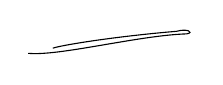
\begin{tikzpicture}[x=0.65cm,y=0.65cm]
\draw[line width=0.4pt] (0,0) .. controls (0.6,-0.06) and (2.15,0.35) .. (3.1,0.38) .. controls (3.25,0.41) and (3.1,0.49) .. (2.9,0.43) .. controls (1.7,0.33) and (0.65,0.16) .. (0.48,0.10);
\end{tikzpicture}}}}
p.24, dernière ligne : dommage qu'on ne do\deleted{t}n\deleted{\unsure{e|a}}ne pas de \deleted{\unsure{m}}démonstration.

p.25, li.8 : ``le soin de'' et non ``de''. Répétition \deleted{\unsure{malsonnante}} de ``développer''.

p.25, li.13 du bas : ``on peut construire $S'$ '' et non ``... $S$''

% archive sheet number: 70
\scanpage{72}
\mspage{\handwritten{7}}

p.25, li.10 du bas : hint pour ``il n'est pas difficile de montrer ...''?

p.26, li.10 : ``dont on peut penser que c'est le même ...'' : y a-t-il \inserted{(dans la situation présente, i.e. $S$ local régulier de pt fermé $s$)} une caractérisation d'un homomorphisme (7.17.4.1) ? \handwritten{(${}^1$)}

p.27, li.1 et 2 du bas : ``au-dessus'' et non ``au dessus''. Dire ``dans le normalisé'' au lieu de ``du normalisé''.

p.28 : dans la bibliographie, manque la référence Abhyankar sur la résolution des singularités des surfaces arithmétiques.

\handwritten{(${}^1$) Est-ce que 7.2 ne \unsure{x|se} généralise pas ?}

% archive sheet number: 71
\scanpage{74}

\begin{flushright}
Massy le 3.11.1970\\
\end{flushright}

\noindent Cher Ferrand,\\

J'aimerais savoir si je peux compter sur ton exposé SGA 6 XI dans un avenir assez rapproché (diso\unsure{l|n|u} d'ici fin décembre). Dans le cas contraire, je pense qu'il serait préfé\deleted{é}r\deleted{\unsure{r}}able que je publie SGA 6 sans l'exposé XI. Il serait quand même raisonnable, après le travail que tu t'es tapé, que tu en fasses au moins un article d'exposition, et j'aimerais savoir alors où tu penses le publier, pour que je puisse y référer dans l'introduction à SGA 6.

Bien cordialement\\

\margin{\handwritten{\figure{\begin{tikzpicture}[x=0.5cm,y=0.5cm]
\draw[line width=0.25pt] (0,0.65) .. controls (0.4,0.46) and (1.12,0.24) .. (1.02,0.05) .. controls (1.00,0.01) and (0.96,0.00) .. (0.94,0.00);
\end{tikzpicture}}}}
% archive sheet number: 73
\scanpage{85}
\mspage{538}

\begin{center}
TABLE DES MATIERES
\end{center}

\noindent AVANT-PROPOS \dotfill

\noindent INTRODUCTION\dotfill

\noindent CHAPITRE \unsure{O|0} .- Préliminaires\dotfill

\noindent\quad \S\ 1. Foncteurs représentables\dotfill

\noindent\qquad 1.1. Foncteurs représentables\dotfill

\noindent\qquad 1.2. Produits fibrés dans une catégorie\dotfill

\noindent\qquad 1.3. Changement de base\dotfill

\noindent\qquad 1.4. Noyaux ; morphisme diagonal\dotfill

\noindent\qquad 1.5. Foncteurs adjoints\dotfill

\noindent\qquad 1.6. Structures algébriques dans les catégories\dotfill

\noindent\qquad 1.7. Morphismes fonctoriels représentables\dotfill

\noindent\quad \S\ 2. Compléments de topologie\dotfill

\noindent\qquad 2.1. Espaces irréductibles\dotfill

\noindent\qquad 2.2. Espaces localement noethériens\dotfill

\noindent\qquad 2.3. Ensembles quasi-constructibles et ensembles constructibles\dotfill

\margin{\handwritten{?}}
\noindent\qquad \deleted{2.4. Fonctions constructibles}\deleted{\mbox{............................}}

\noindent\qquad \deleted{2.5.}

\noindent\qquad 2.4. Ensembles constructibles dans les espaces noethériens

\noindent\qquad 2.5? Fonctions constructibles\dotfill

\noindent\qquad 2.6. Parties très denses d'un espace topologique\dotfill

\noindent\qquad 2.7. Quasi-homéomorphismes\dotfill

\noindent\qquad 2.8. Espaces de Jacobson\dotfill

\noindent\qquad 2.9. Espace sobre associé à un espace topologique\dotfill

\noindent\qquad 2.10.Applications ouvertes en un point \dotfill

\noindent\quad \S\ 3. Compléments sur les faisceaux\dotfill

\noindent\qquad 3.1. Faisceaux à valeurs dans une catégorie\dotfill

\noindent\qquad 3.2. Préfaisceaux sur une base d'ouverts\dotfill

\noindent\qquad 3.3. Recollement de faisceaux\dotfill

\noindent\qquad 3.4. Images directes de préfaisceaux\dotfill

\noindent\qquad 3.5. Images réci\deleted{\unsure{r}}p\deleted{p}roques de préfaisceaux\dotfill

\noindent\qquad 3.6. Faisceaux simples et faisceaux localement simples\dotfill

\noindent\qquad 3.7. Images réciproques de faisceaux de groupes ou d'anneaux\dotfill

% archive sheet number: 84
\scanpage{86}
\mspage{541}

\noindent\qquad 3.8. Morphismes universellement ouverts , universellement fermés , universellement bicontinus\dotfill

\noindent\qquad 3.9. Morphismes générisants\dotfill

\noindent\qquad 3.10. Morphismes submersifs et universellement submersifs

\noindent\quad \S\ 4. Sous-schémas et morphismes d'immersion .\unsure{\textsubscript{.}} Schémas réduits\dotfill

\noindent\qquad 4.1. Sous-schémas\dotfill

\noindent\qquad 4.2. Morphismes d'immersion\dotfill

\noindent\qquad 4.3. Image réciproque d'un sous-schéma\dotfill

\noindent\qquad 4.4. Immersions locales et isomorphismes locaux\dotfill

\noindent\qquad 4.5. Schémas réduits\dotfill

\noindent\qquad 4.6. Existence d'un sous-schéma d'espace sous-jacent donné\dotfill

\noindent\quad \S\ 5. Morphismes séparés . Critères valuatifs\dotfill

\noindent\qquad 5.1. Diagonale d'un $S$-schéma\dotfill

\noindent\qquad 5.2. Morphismes et schémas séparés\dotfill

\noindent\qquad 5.3. Critères \deleted{\unsure{a|e}}de séparation\dotfill

\noindent\qquad 5.4. Morphismes schématiquement dominants et sous-schémas schématiquement denses\dotfill

\noindent\qquad 5.5. Critères valuati\deleted{\unsure{s|b}}fs\dotfill

\noindent\quad \S\ 6. Conditions de finitude relatives\dotfill

\noindent\qquad 6.1. Morphismes quasi-compacts et morphismes quasi-séparés\dotfill

\noindent\qquad 6.2. Morphismes localement de type fini et morphismes localement de présentation finie\dotfill

\noindent\qquad 6.3. Morphismes de type fini et morphismes de présentation finie\dotfill

\noindent\qquad 6.4. Schémas de \deleted{d}Jacobson et anneaux de \deleted{j}Jacobson\dotfill

\noindent\qquad 6.5. Schémas algébriques et localement algébriques\dotfill

\noindent\qquad 6.6. Détermi\deleted{j}nation locale d'un morphisme\dotfill

\noindent\qquad 6.7. Image directe d'un faisceau quasi-cohérent\dotfill

\noindent\qquad 6.8. Prolongement de sections de faisceaux quasi-cohérents

\noindent\qquad 6.9. Prolongement des faisceaux quasi-cohérents\dotfill

\noindent\qquad 6.10.Image schémat\deleted{\unsure{l|t}}ique d'un schéma\unsure{,|.} Adhérence schématique d'un sous-schéma\dotfill

\noindent\qquad 6.11.Morphismes quasi-finis\dotfill

% archive sheet number: 85
\scanpage{87}
\mspage{539}

\noindent\qquad 3.8. Quasi-homéomorphismes et images réciproques de faisceaux\dotfill

\noindent\qquad 3.9. Faisceaux d'espaces pseudo-discrets\dotfill

\noindent\quad \S\ 4. Espaces annelés\dotfill

\noindent\qquad 4.1. Espaces annelés , $A$-Modules , $A$-Algèbres\dotfill

\noindent\qquad 4.2. Image directe d'un $A$-Module\dotfill

\noindent\qquad 4.3. Image réciproque d'un $B$-Module\dotfill

\noindent\qquad 4.4. Relations entre images directes et images réciproques\dotfill

\noindent\qquad 4.5.Immersions ouvertes et morphismes représentables par des immersions ouvertes \dotfill

\noindent\quad \S\ 5. Faisceaux quasi-cohérents et faisceaux cohérents\dotfill

\noindent\qquad 5.1. Faisceaux quasi-cohérents\dotfill

\noindent\qquad 5.2. Faisceaux de type fini\dotfill

\noindent\qquad 5.3. Faisceaux cohérents\dotfill

\noindent\qquad 5.4. Faisceaux localement libres\dotfill

\noindent\qquad 5.5. Modules localement libres sur un espace localement annelé\dotfill

\noindent\qquad 5.6. Groupe de Picard\dotfill

\noindent\qquad 5.7. Morphismes plats d'espaces annelés\dotfill

\noindent\quad \S\ 6. Compléments d'algèbre commutative .

\noindent\qquad 6.1. Limites inductives d'anneaux\dotfill

\noindent\qquad 6.2. Identification du module $M_f$ à une limite \deleted{\unsure{project|projecti}} inductive\dotfill

\noindent\qquad 6.3. Propriétés de finitude\dotfill

\noindent\qquad 6.4. Critères pour qu'un anneau soit noethérien\dotfill

\noindent\qquad 6.5. Anneaux normaux et ferm\deleted{t}e\deleted{e}ture intégrale\dotfill

\noindent\qquad 6.6. Compléments sur la platitude\dotfill

\noindent\qquad 6.7. Compléments sur\deleted{\unsure{l|1}} les modules projectifs\dotfill

\noindent\qquad 6.8. Existence d'extensions plates d'anneaux locaux\dotfill

\noindent\quad \deleted{\S\ \unsure{7.}}

\noindent\quad \S\ 7. Compléments d'algèbre topologique\dotfill

\noindent\qquad 7.1. Anneaux admissibles\dotfill

\noindent\qquad 7.2. Anneaux adiques et limites projectives\dotfill

\noindent\qquad 7.3. Anneaux préadiques noethériens\dotfill

\noindent\qquad 7.4. Modules quasi-finis sur les anneaux locaux\dotfill

\noindent\qquad \deleted{7\unsure{.}} 7.5. Anneaux de séries formelles restreintes\dotfill

\noindent\qquad 7.6. Anneaux complets de fractions\dotfill

% archive sheet number: 86
\scanpage{88}
\mspage{540}

\noindent\qquad 7.7. Produits tensoriels complétés\dotfill

\noindent\qquad 7.8. Topologies sur les modules d'homomorphismes\dotfill

\noindent CHAPITRE I .- Le langage des schémas\dotfill

\noindent\quad Sommaire\dotfill

\noindent\quad \S\ 1. Schémas affines\dotfill

\noindent\qquad 1.1. Le spectre premier d'un anneau\dotfill

\noindent\qquad 1.2. Propriétés fonctorielles des spectres premiers d'anneaux\dotfill

\noindent\qquad 1.3. Faisceau associé à un module\dotfill

\noindent\qquad 1.4. Faisceaux quasi-cohérents sur un spectre premier\dotfill

\noindent\qquad 1.5. Faisceaux cohérents sur un spectre premier\dotfill

\noindent\qquad \deleted{S}1.6.Schémas affines et morphismes d'espaces localement annelés dans des schémas affines\dotfill

\noindent\qquad 1.7.Images directes et images réciproques de faisceaux quasi-cohérents par des morphismes de schémas affines\dotfill

\noindent\quad \S\ 2. Schémas et morphismes de schémas\dotfill

\noindent\qquad 2.1. Définition des schémas\dotfill

\noindent\qquad 2.2. Faisceaux quasi-cohérents sur un schéma\dotfill

\noindent\qquad 2.3. Morph\deleted{\unsure{u|n}}ismes de schémas\dotfill

\noindent\qquad 2.4. Recollement de schémas\dotfill

\noindent\qquad 2.5. Schémas locaux\dotfill

\noindent\qquad 2.6. Schémas au-dessus d'un schéma\dotfill

\noindent\qquad 2.7. Schémas noethériens et schémas localement noethériens\dotfill

\noindent\qquad 2.8. Schémas artiniens\dotfill

\noindent\quad \S\ 3. Produit et somme de schémas. Changement de base\dotfill

\noindent\qquad 3.1. Somme de schémas\dotfill

\noindent\qquad 3.2. Produit de schémas\dotfill

\noindent\qquad 3.3. Produit tensoriel de Modules quasi-cohérents sur un produit de schémas\dotfill

\noindent\qquad 3.4. Changements de base ; fibres\dotfill

\noindent\qquad 3.5. Points d'un schéma à valeurs dans un schéma ; points géométriques\dotfill

\noindent\qquad 3.6. Morphismes surjectifs\dotfill

\noindent\qquad 3.7. Morphismes radiciels\dotfill

% archive sheet number: 87
